\vssub
\subsubsection{~球面多单元（SMC）网格} \label{sub:num_space_SMC}
\opthead{SMC}{\ws (MetOffice)}{J.-G. Li}

\noindent
球面多单元（SMC）网格 \citep{art:Li11} 是 Cartesian 多单元网格 \citep{art:Li03} 向球坐标系统的扩展。它是一种非结构网格，但保留了常规经纬度网格单元，因此球坐标上的所有传播公式仍然适用，相应地所有有限差分格式也仍可使用。SMC 网格以类似于削减网格 \citep{art:RA94} 的方式放宽高纬度地区的 CFL 限制。通过转为积分方程，引入极区单元以消除微分输运方程的极点奇异性。上游非振荡二阶（UNO）平流格式 \citep{art:Li08} 已在 SMC 网格上实现，用于空间传播和谱间传播。UNO2 格式可通过 {\F PSMC} namelist 逻辑变量 {\code UNO3} 替换为三阶格式。UNO3 格式类似于 UQ 格式，但把其通量限制器替换为 UNO2 格式。波浪折射诱导旋转和大圆转向采用一种简单旋转格式 \citep{art:Li12}。对于任意时间步长，折射格式都是无条件稳定的，但最大折射诱导旋转角受到朝向局地梯度方向的最大可能折射角限制。除这一物理限制器外，{\F PSMC} namelist 中还有用户定义参数 {\code RFMAXD}，用于限制每个时间步的最大折射角。其默认值为 36.0 度。为减轻 garden sprinkler effect，使用类似 \cite{art:BH87} 的扩散项，但扩散系数简化为单一均匀参数（式~(\ref{eq:Dnn_d}) 中的 $D_{nn}$）。还可通过 {\F PSMC} namelist 逻辑变量 {\code AVERG} 使用附加的 1-2-1 加权平均格式。与常规网格相比，SMC 网格可显著减少计算时间，这得益于高纬度时间步限制的放宽以及从模式中移除陆点。为修正高纬度地区无效的标量假设，提供了一种补救方法，可将全球波浪模式扩展到整个北冰洋 \citep{art:Li16}。该 Arctic 部分可通过设置 {\F PSMC} namelist 参数 {\code Arctic=.TRUE.} 激活。

SMC 网格可用于替代规则经纬度网格，使模式区域可扩展到高纬度甚至北极，而无需缩短时间步长。除准备少量额外输入文件（包括单元数组和面数组文件）外，该应用对规则网格模式只需少量修改。单元数组可利用已有规则网格水深，仅使用海点，并在若干纬度带沿经向合并单元来生成 \citep{art:Li11}。

SMC 网格的另一个重要用途是构建多分辨率网格。基础层级 SMC 网格单元可通过把经度和纬度网格长度减半，细化为 4 个四分之一单元。该细化层级上的任意单元又可进一步划分为另外 4 个四分之一单元。这种细化可按需要继续，从而形成若干细化层级上的多分辨率网格。为保持一致，单分辨率 SMC 网格被视为只有一个层级。常规规则网格输入文件，如水深、陆海掩膜和子网格阻挡，不再需要，取而代之的是仅含海点的单元和面数组，以及一个子网格阻挡文件。水深作为整数米值存储在单元数组最后一列（第 5 列）。掩膜将在 ww3\_grid 内部用仅含海点的单元数组定义。

风和海流（若有）强迫可默认使用基础分辨率上的规则网格，作为任意 SMC 网格（单层或多层）的输入强迫。它将在模式内部插值到细化层级（若有）上。SMC 网格还可通过 {\F PSMC} namelist 中的 {\code SEAWND} 逻辑变量开启仅海点风和流输入选项。该仅海点选项不仅免除了模式内部对风（以及流，若有）插值的需要，还允许混合不同分辨率的风（以及流）强迫，并直接插值到多分辨率单元上，使其成为真正的多分辨率模式。

\begin{figure}
\centerline{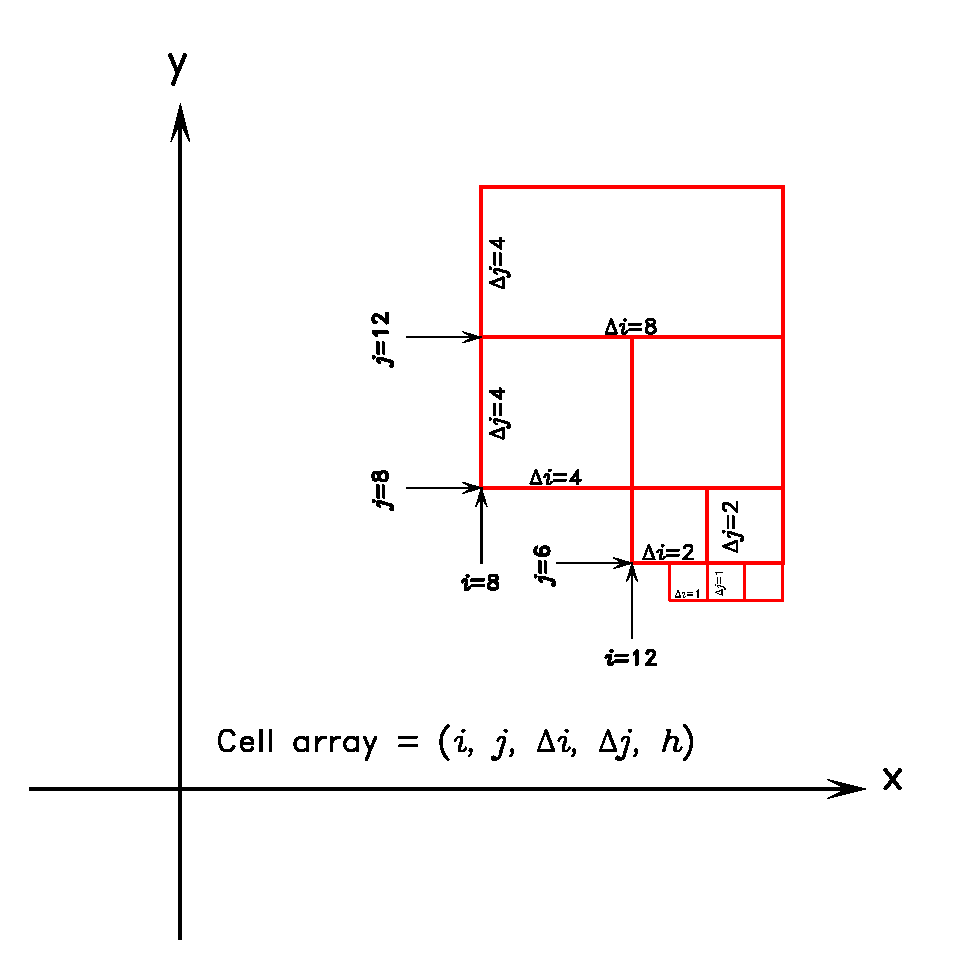
\epsfig{file=./num/smcelary.eps,angle=0,width=3.in}}
\caption{SMC 网格中使用的单元数组示意。}
\label{fig:SMCells} \botline
\end{figure}

SMC 网格的一个重要特征是它是非结构网格，也就是说，单元不要求按照其物理位置相邻排列。为便于多分辨率 SMC 网格，单元按其大小排序，使给定层级上的单元聚集在一个子循环中，共用一个子时间步。细化层级子步的基础层级时间步随网格长度一起减半。这有效避免了模式因细化单元的 CFL 限制而变慢。传播格式所需的相邻单元信息由单元面数组提供，这些面数组会针对给定单元数组列表预先计算。因此，不需要把仅含海点的 SMC 网格单元扩展到完整网格上进行传播。图~\ref{fig:SMCells} 展示了 SMC 单元数组的定义方式，图~\ref{fig:SMC_Arctic} 展示了 6-12-25 km 三层 SMC 网格中的北极区域。金色和红色圆圈分别标记 SMC6-25 网格中的全球部分和北极部分。金色圆圈内的北极部分需要固定参考方向来定义其波向箱。全球部分（直到金色圆圈）可在没有北极部分的情况下独立运行。如果用 ARC 选项激活北极部分，则从红色圆圈到金色圆圈的 4 行会在北极部分中复制为边界单元。北极部分使用单独的单元和面数组，并在波浪模式中并入全球数组用于传播。对于带输入边界条件的区域 SMC 网格，需要提供边界单元序号列表，并由 {\F PSMC} namelist 参数 {\code NBISMC} 指定边界单元数量。SMC 网格使用与规则经纬度网格相同格式的边界输入文件。边界文件可由规则网格或全球 SMC 网格模式生成，方法与规则网格一样指定边界单元中心位置。

\begin{figure}
\centerline{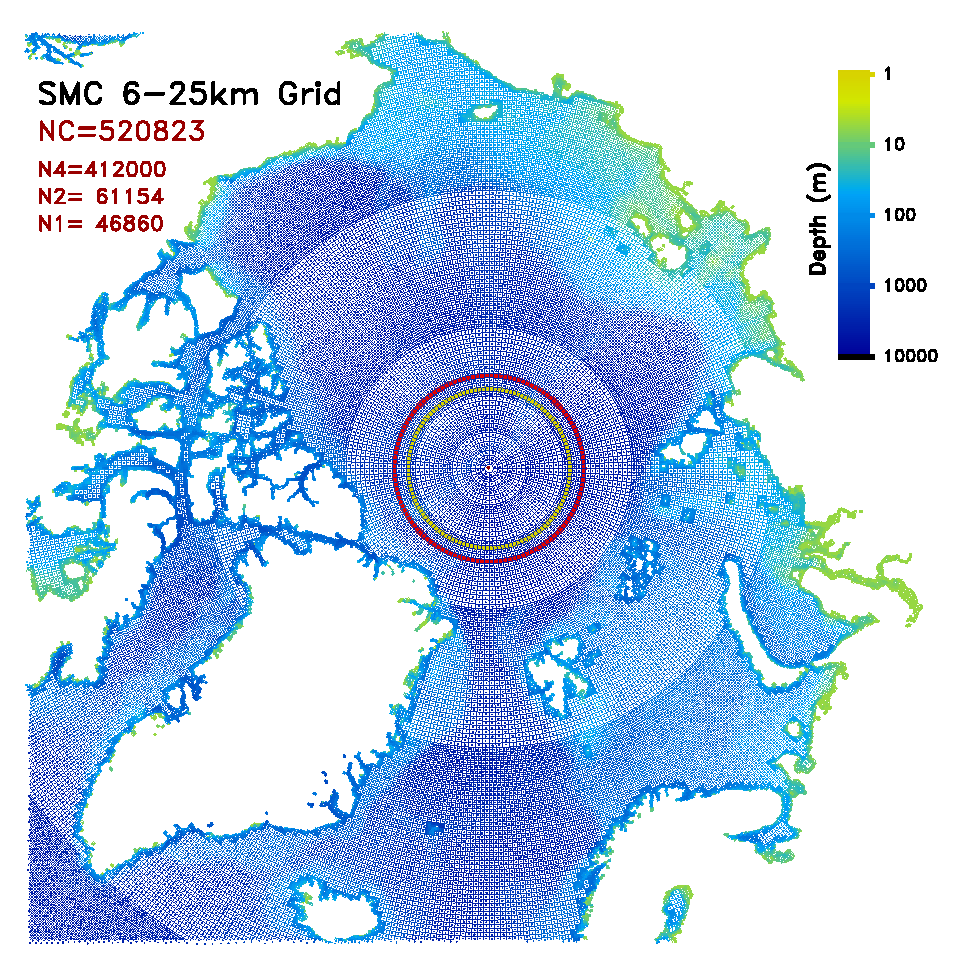
\epsfig{file=./num/JCP_Fig2_GArc.eps,angle=0,width=4.in}}
\caption{6-12-25km 多分辨率 SMC 网格中的北极区域。}
\label{fig:SMC_Arctic} 
\botline
\end{figure}

已开发若干 IDL 和 F90 程序，用于生成 SMC 网格单元和面数组，以及可视化网格网格和波场，但它们尚未正式纳入 WW3 软件包。smc\_docs/SMCG\_TKs/ 中提供了一个 IDL 程序 (Glob50SMCels.pro)，用于使用规则 50 km 网格水深文件 (G50kmBathy.dat) 生成全球 50km SMC 网格。面数组由两个 F90 程序生成，一个用于全球部分 (G50SGlSide.f90)，另一个用于北极部分 (G50SAcSide.f90)。由于极区单元的特殊处理 \citep{art:Li12}，北极极点单元的面数组需要采用不同于其他单元的方法。单元数组文件必须先用一个简单 Linux 脚本 (countcells) 排序，然后再输入面数组生成程序。面数组也需要用 Linux 脚本 (countijsd) 排序，以确定多层级子循环计数。可运行一个独立谱传播测试 (G50SMCSRGD.f90) 来测试单元和面数组，其输出可用 IDL 脚本 g50smstrspb.pro 可视化；该脚本使用 SMC 网格可视化程序 g50smcgrids.pro 保存的投影文件。通过修改 g50smcgrids.pro 中的投影参数，用户可选择投影视点（以经纬度度数表示），并保存投影供模式输出可视化使用。子网格阻挡文件可由 IDL 程序 Glob50SMCObstr.pro 生成。

SMC 网格选项的编译类似于规则经纬度网格，但需要额外开关 {\code SMC} 来调用 SMC 网格。由于 SMC 网格与规则经纬度网格共享若干网格变量，也应选择规则网格开关，例如 {\code PR2 UNO} 或 {\code PR3 UQ}。SMC 网格类型 {\code SMCTYPE} 通过在 ww3\_grid.inp 文件中用 {\code SMCG} 替换 {\code RECT} 来定义。注意，SMC 网格构建在规则经纬度网格内部，因此在 ww3\_grid.inp 文件中仍需基础分辨率层级上的规则经纬度网格参数，如 NX、NY、SX、SY、X1 和 Y1。规则经纬度网格水深、陆海掩膜和子网格阻挡输入文件不再需要，它们由 SMC 网格仅海点文件替代（水深存储在单元数组中，子网格阻挡存储在 G50GObstr.dat 中）。不过，ww3\_grid.inp 中的水深和陆海掩膜输入行会保留，用于传递最小水深等参数。由于高纬度处的合并以及可能存在的细化分辨率，规则网格映射数组会为与 SMC 网格单元保持一致而略作修改。三层 Lake Erie SMC 网格模式示例见回归测试 \emph{regtests/ww3\_tp2.10}。

SMC 网格模式的输出后处理已针对 ww3\_ounf 和 ww3\_outf 开发。对于 ww3\_ounf，用户可选择在原生模式网格海点上提取多分辨率信息，或在模式网格定义中设置的任一分辨率层级上生成规则网格。ww3\_outf 程序处理 SMC 网格数据时，可输出为基础分辨率层级上完全展开的规则经纬度网格输出，也可输出为所有 SMC 网格海点处的 ASCII 输出（type-4）。对于规则网格输出，参数值由所有与所选输出单元边界重叠的 SMC 网格单元作面积加权平均确定。海点数据的纬度和经度对应原生模式网格单元中心。对于 ww3\_ounf 海点输出，netCDF 文件中还提供描述单元大小的变量。

本代码版本未提供海点输出的可视化工具；不过，可根据请求从 Met Office 获得一些示例。针对 netCDF 海点输出，已开发一个基于 python 的 GUI 工具。所有单元 ASCII 输出可借助输入单元数组文件进行可视化，因为输出单元顺序与输入单元数组相同。IDL 脚本 g50smcswhglb.pro 是绘制全球 50km SMC 网格 SWH 输出的示例程序。它使用 g50smcgrids.pro 生成的投影文件。鼓励用户用其他语言开发自己的网格生成和后处理程序。一个 Python 小组已经成立，用于开发 SMC 网格单元和面数组生成及可视化程序。这些新的 Python 程序目前存放在一个单独的 github 站点：  
\url{https://github.com/ww3-opentools/ww3-grid/}
该站点仍处于开发阶段。欢迎 WW3 Python 程序员测试并为其改进作贡献。

从第 7 版起，SMC 网格扩展为可在 WW3 多网格模式下运行。目前，它只支持同等级 SMC 子网格并行运行。SMC 子网格的生成方式类似于具有自身边界单元列表的单个区域 SMC 网格。建议边界单元采用来自相邻子网格的复制单元，因为 SMC 子网格的边界谱交换为整谱复制粘贴，即不需要插值。规则经纬度子网格也可加入同一等级的 SMC 子网格组，但边界条件仍限于整谱交换。原始经纬度网格边界插值未启用。该简化减少了 MPI 通信负载，但如果边界单元中心未对齐，可能会损失一些精度。Great Lakes 的 SMC 子网格示例见回归测试 \emph{regtests/mww3\_test\_09}。它以 3 个 SMC 层级（0.5-1-2 km）覆盖 Lake Michigan、Huron 和 Superior，并尽量减少边界连接。
  
SMC 网格支持混合并行化；在 Cray XC40 超级计算机上使用 3 或 6 个 OpenMP 线程运行时，总耗时可减少一半。进一步增加 OpenMP 线程似乎效果不大。混合并行和多网格并行相结合，可使 \emph{mww3\_test\_09} 中 3 个 Great Lake 子网格的计算机使用规模扩展到 100 个以上节点。

建议阅读 smc\_docs/SMC\_Grid\_Guide.pdf 或会议网页上的会议论文 \citep{tol:LiS17}：
http://www.waveworkshop.org/15thWaves/
以获取更多信息；关于 SMC 网格的任何帮助，也可联系 \url{Jian-Guo.Li@metoffice.gov.uk}。

